%!Mode:: "TeX:UTF-8"
%!TEX encoding = UTF-8 Unicode
%!TEX language=zh
%arara: xelatex
\documentclass{ctexart}
\newif\ifpreface
%\prefacetrue
\input{../../../global/all}
\usepackage{tikz}
\usepackage{tkz-euclide}
\newcommand{\diag}{\mathrm{diag}}
\newcommand{\norm}[1]{\lVert#1\rVert}
\newcommand{\res}[2]{#1|_{#2}}
\begin{document}
\large
\setlength{\baselineskip}{1.2em}
\ifpreface
    \input{../../../global/preface}
\newgeometry{left=2cm,right=2cm,top=2cm,bottom=2cm}
\else
\newgeometry{left=2cm,right=2cm,top=2cm,bottom=2cm}
\maketitle
\fi
%from_here_to_type

\begin{problem} 
  Let \(A_1=B^{-1}C \) and \(A_2 =CB \) where \(C \) is a Hermitian matrix and 
  \(B \) is a Hermitian Positive Definite matrix. 
  \begin{enumerate}
    \item Are \(A_1 \) and \(A_2 \)   Hermitian in general? 
\item   Show that \(A_1 \) and \(A_2 \) are Hermitian (self-adjoint)
  with respect to the \(B \)-inner product.
  \end{enumerate}
\end{problem}
\begin{solution}
  \begin{enumerate}
    \item No, in fact \(A_1, A_2 \) are Hermitian \(\iff BC=CB \).

      ``\(\implies\)'': Since \(A_1,A_2 \) are Hermitian, we can obtain 
      \(A_1^H=(B^{-1}C)^H=C^H(B^{-1})^H=C^H(B^H)^{-1} =B^{-1}C=A_1\), 
      \(A_2^H=(CB)^H=B^HC^H =CB=A_2\). Besides, since \(B,C \) are Hermitian, we 
      get \(B^H=B,C^H=C \). Thus, \(A_1^H=C^H(B^H)^{-1}=CB^{-1}=B^{-1}C,A_2^H=BC =CB\).

      ``\(\impliedby\)'':According to the statement above, we can get 
      \(A_1^H=CB^{-1},A_2^H=CB \). Since \(BC=CB \), we can get 
      \(CB^{-1}=B^{-1}C \). Thus, \(A_1^H=CB^{-1} = B^{-1}C=A_1\), \(A_2^H=BC=CB \).
    \item First, we need to prove \(B \)-inner product is well-defined.
      We define \(B \)-inner product as below. 
      Let \(\langle x,y\rangle:=y^HBx, \forall x,y \in \mathbb{C}^n  \), where \(B,C \in \mathbb{C}^n \).
      \begin{itemize}
        \item \(\forall x_1,x_2, y \in \mathbb{C}^n \), \(\langle \lambda_1 x_1 + \lambda_2 x_2 ,y\rangle =y^HB(\lambda_{1}x_1 + \lambda_2 x_2)=\lambda_1y^H B x_1 + \lambda_2 y^H B x_2 =
          \lambda_1 \langle x_1,y\rangle + \lambda_2\langle x_2,y\rangle\).
        \item \(\forall x,y \in \mathbb{C}^n \),\(\langle y,x \rangle =x^HBy=(y^T B^T \overline{x})^T=\overline{(y^HB^Hx)^T}=\overline{y^HB^Hx}=\overline{y^HBx}=\overline{\langle x,y\rangle }\), 
          since \(B \) is Hermitian.
        \item \(\forall x \in \mathbb{C}^n \setminus \{0\} \),\(\langle x,x\rangle =x^HBx>0 \), since \(B \) is Positive Definite. 
      \end{itemize}
     Next, we will prove \(A_1,A_2 \) are self-adjoint under \(B \)-inner product.
     \begin{itemize}
       \item \(A_1 \) is self-adjoint: \(\forall x,y \in \mathbb{C}^n \), \(\langle A_1x,y\rangle =y^HBA_1x =y^HB(B^{-1}C)x=y^HCx\). 
         \(\langle x,A_1y\rangle =(A_1y)^HBx=y^HA_1^HBx=y^HCB^{-1}Bx=y^HCx \). Thus, \(\langle A_1x,y\rangle =\langle x,A_1y\rangle  \).
       \item \(A_2 \) is self-adjoint:\( \forall x,y \in \mathbb{C}^n\),\(\langle A_2x,y\rangle =y^HBA_2x=y^HB(CB)x \).
         \(\langle x,A_2y\rangle =(A_2y)^HBx=y^HA_2^HBx=y^HBCBx \). Thus, \(\langle A_2x,y\rangle =\langle x,A_2y\rangle  \).
     \end{itemize}
  \end{enumerate}
\end{solution}

\begin{lemma}\label{lem:1.13}
  If a normal matrix is triangular, then it is a diagonal matrix.
\end{lemma}
\begin{problem} 
  \begin{enumerate}
    \item \label{ite:2.1} Let a matrix \(A \) be such that \(A^H =p(A) \), where \(p \) is a polynomial. 
  Show that \(A \) is normal. 
\item \label{ite:2.2}   Given a diagonal complex matrix \(D \), show 
  that there exists a polynomial of degree \(< n \) such that \(\overline{D} =p(D ) \). 
\item \label{ite:2.3}   Use \ref{ite:2.2} to show that a normal matrix satisfies \(A^H=p(A) \) for a certain 
  polynomial of \(p \) of degree \(<n \). 
\item \label{ite:2.4}   As an application, use \ref{ite:2.3}  to 
  provide an alternative proof of lemma \ref{lem:1.13}. 
  \end{enumerate}
\end{problem}
\begin{solution}
 \begin{enumerate}
   \item Let matrix \(A \) satisfy \(A^H = p(A) \), where \(p(x):=\sum_{i=0}^{n}a_ix^i,a_i \in \mathbb{C},0 \leq i \leq n \).
     Then \(p(A)=\sum_{i=0}^{n}a_iA^i \). So \(A^HA=(\sum_{i=0}^{n}a_iA^i)A=\sum_{i=0}^{n}a_iA^{i + 1}=A(\sum_{i=0}^{n}a_iA^i)=Ap(A)=AA^H \).
   \item Assume \(D=\diag(\lambda_1,\cdots,\lambda_n), \lambda_i \in \mathbb{C}, 1 \leq i \leq n  \). 
     First, we need to prove \(\forall f \) is a polynomial, \(f(D)=\diag(f(\lambda_1),\cdots,f(\lambda_n)) \).
     Assuming \(f(x)=\sum_{i=0}^{m}a_ix^i,a_i \in \mathbb{C},0 \leq i \leq m \), we get\( f(D)=\sum_{i=0}^{m}a_iD^i=\sum_{i=1}^{m}a_i \diag(\lambda_1^i,\cdots,\lambda_n^i)=
     \sum_{i=0}^{m}\diag(a_{i}\lambda _1^i,\cdots,a_i \lambda _n^i)=\diag(\sum_{i=0}^{m}a_{i}\lambda _1^i,\cdots,\sum_{i=0}^{m}a_i \lambda _n^i)=\diag(f(\lambda_1),\cdots,f(\lambda_n))\). 
     
     Next, since \(\overline{D} =\diag(\overline{\lambda_1},\cdots,\overline{\lambda_n}) \) and we need to find a polynomial \(p(x)\) with degree \(<n \) 
     satisfying \(\overline{D}=\diag(\overline{\lambda_1},\cdots,\overline{\lambda_n})=\diag(p(\lambda_1),\cdots,p(\lambda_n)) \), 
     we can turn to find a polynomial \(p(x) \) satisfying \(\forall 1 \leq i \leq n \), \(\overline{\lambda_i}=p(\lambda_i) \) with degree \(<n \). 
     By Lagrange interpolation method, let \[ p(x)=\sum_{i=1}^{n}\overline{\lambda_i}\prod_{1 \leq j \leq n, j \neq i} \frac{x-\lambda_j}{\lambda_i-\lambda_j}=:\sum_{i=1}^{n}\overline{\lambda_i}L_i(x) .\] 
     Since \(\forall 1 \leq i \leq n \), \(L_i(\lambda_i)=\prod_{1 \leq j \leq n, i \neq j}\frac{\lambda_i-\lambda_j}{\lambda_i-\lambda_j}=1 \), \( \forall k \neq i, 1 \leq k \leq n,\) 
     \[
       \begin{aligned}
         L_i(\lambda_k)=&\prod_{1 \leq j \leq n, j \neq i} \frac{\lambda_k-\lambda_j}{\lambda_i-\lambda_j}\\
         =&\prod_{1 \leq j \leq n, j \neq i,k} (\frac{\lambda_k-\lambda_j}{\lambda_i-\lambda_j}) \frac{\lambda_k-\lambda_k}{\lambda_i-\lambda_j}\\
         =&0 
       \end{aligned}
      \]
      we can get \(p(\lambda_i)=\sum_{k=1}^{n}\overline{\lambda_k}L_k(\lambda_i)=\sum_{1 \leq k \leq n, k \neq i}\overline{\lambda_k} L_k(\lambda_i) + \overline{\lambda_i}L_i(\lambda_i)=\overline{\lambda_i} \).
      Besides, since \(\forall 1 \leq i \leq n \), \( \deg(L_i(x)) \leq n -1\), we can know that \(\deg(p(x))=\max\{\deg(L_i(x)):1 \leq i \leq n\} \leq n-1 <n\). 
      Therefore, \(p(x) \) is what we want.
    \item First, for preparation, we will prove the lemma below: 
      \begin{lemma}\label{lem:normal}
        \(V \) is an \(n \)-dimension linear space on \(\mathbb{C} \), \(A \) is a linear operator on \(V \), 
        then \(\exists v \in V\setminus\{0\} , \norm{v}=1 , \lambda \in \mathbb{C}\) satisfying \(Av=\lambda v \).
      \end{lemma}
     \begin{proof}
      Let \(p(x)=|A-xI| \), then \(p(x) \in \mathbb{C}[x] \), \(\deg p =n \). Since \(\mathbb{C} \) is algebraically closed, we can get \(\lambda \in \mathbb{C}  \) such that 
       \(p(\lambda )=0 \). Thus, the linear function \((A-\lambda I)x=0 \) has nonzero solution \(w \).
       Let \(v:=\frac{w}{\norm{w}} \), then \(0=(A-\lambda I)w=(A-\lambda I)(\norm{w}v) \). Therefore, \(Av=\lambda v \).
     \end{proof}
    %  \begin{lemma}\label{lem:org}
    %    \(v,u \) are 2 eigenvectors of a normal matrix \(A \) corresponding to 2 different eigenvalues \(\lambda_1,\lambda_2 \). 
    %    Then \(\langle u,v\rangle =0 \).
    %  \end{lemma}
    % \begin{proof}
    %   
    % \end{proof}
     
     Next, we will prove \(A \) is an \(n \)-dimension normal matrix, then \(\exists U \) such that \(U^H U=I \) and \(U^H AU=\Lambda \), where \(\Lambda \) is diagonal.
     According to lemma \ref{lem:normal}, \(\exists v_1, \lambda_1 \) satisfies \( \norm{v_1} =1, Av_1=\lambda_1v_1 \).
     Consider \(W_1:=span\{v_1\}, V_1:=\{x \in \mathbb{C}^n: \langle x,v\rangle =0, \forall v \in W_1\} \). Then \(\dim V_1 =n-1 \). 
     Since \(A \) is normal, \(AA^H=A^HA \), we can get \(AA^Hv_1=A^HAv_1=\lambda_1A^Hv_1 \). Thus, \(A^Hv_1 \in W_1 \).
     Otherwise, \(A^Hv_1=kv_1 + w \), \(k \in \mathbb{C}, w \in V_1\setminus \{0\} \). Then \(A(A^Hv_1)=A(kv_1 + w)=\lambda_1 (kv_1) + Aw=\lambda_1(kv_1 + w) \). 
     So \(Aw=\lambda_1w \). That means \(w \in W_1 \). Then \(\langle w,w\rangle =0 \), contradiction.
     So \(\forall v \in V_1 \), \(\langle Av,v_1\rangle =\langle v,A^Hv_1\rangle =0 \). Thus, \(Av \in V_1 \). 
     Let \(A_1:=\res{A}{V_1}: V_1 \to V_1 \) is a linear operator. By lemma \ref{lem:normal}, we can obtain \(v_2 \in V_1 \) is an eigenvector of \(A \) 
     with eigenvalue \(\lambda_2 \).
     We can repeat the process until \(\dim V_n =0 \), which means \(A \) has \(n \) different unit eigenvectors orthogonal to each other, noted 
     as \(\{v_1,\cdots,v_n\} \).
     Let \(U=(v_1,\cdots,v_n) \), then \(U^HU=I \), \(U^HAU=\diag(\lambda_1,\cdots,\lambda_n)=:D  \).

     Finally, let \(p(x) \) taken in the same way when solving \ref{ite:2.2}, so \(\deg p \leq n-1 <n \).
     Then we will prove \(A^H=p(A) \).
     So by \ref{ite:2.2}, we can get \(\overline{U^HAU}=\overline{D}=p(D)=p(U^HAU) \). Since \(U^HU=UU^H=I \), we can get that
    \( p(U^HAU)=U^Hp(A)U\). Besides, \(\overline{U^HAU}=(U^T \overline{A} \overline{U} )^T=U^HA^HU \). Thus, \(U^HA^HU=U^Hp(A)U \). 
     Therefore, \(A^H=p(A) \).
   \item Let \(A \) be normal and triangular. Without loss of generality, we can assume \(A \) is upper triangular. 
     By \ref{ite:2.3}, we can get \(\exists p \) is a polynomial such that \(A^H=p(A) \). Since \(p(A) \) is upper triangular, 
     \(A^H \) is lower triangular, we can know \(A^H \) is diagonal. Therefore, \( A\) is diagonal. 
 \end{enumerate}
\end{solution}

\begin{problem}  
  Let \(A \) be an \(M \)-matrix and \(u,v \) are two nonnegative vectors such 
  that \(v^T A^{-1} u <1 \). Show that \(A-uv^T \) is an \(M \)-matrix.
\end{problem}
\begin{solution}
 Actually, we can  re-definite \(M\)-matrix. First, we will prove \(A \) is \(M \)-matrix \(\iff \) \(a_{ij} \leq 0, i \neq j, i,j =1,\cdots,n \) 
  and \(A^{-1} \geq 0 \).
  ``\(\implies\)'': Obviously true. Only need to prove ``\(\impliedby\)'': Since \(A^{-1} \) exists, we can get \(A \) is nonsigular. 
  Since \(A^{-1}A=I \), we can get \(\forall 1 \leq i \leq n, \sum_{k=1}^{n}a_{ik}b_{ki}=1\), where \(A=(a_{ij}), A^{-1}=(b_{ij}) \). Since \(a_{ik} \leq 0, k \neq i , b_{ik} \geq 0,k \neq i \), 
  we can obtain that \(a_{ik}b_{ik} \leq 0, k \neq i \).
  Thus, we can get \(\sum_{k=1}^{n}a_{ik}b_{ik}=\sum_{1 \leq k \leq n, k \neq i}a_{ik}b_{ik} + a_{ii}b_{ii} =1 \), so \(1-\sum_{1 \leq k \leq n, k \neq i}a_{ik}b_{ik}=a_{ii}b_{ii}\geq 1 \). 
  Since \(b_{ii} \geq 0 \) and \(a_{ii}b_{ii} \geq 1 \), we can get \(b_{ii}>0 \) and \(a_{ii}>0 \). 

  Next, we will prove \((A-u^T)^{-1}=A^{-1} + \frac{A^{-1}uv^TA^{-1}}{1-v^TA^{-1}u} \). Since \(A-uv^T=A(I-A^{-1}uv^T) \), we can consider the inverse of \(I-A^{-1}uv^T \) first. 
  We can formally compute the inverse of \((I-A^{-1}uv^T) \):
  \[
    \begin{aligned}
      (I-A^{-1}uv^T)^{-1}=&\sum_{k=0}^{\infty}(A^{-1}uv^T)^k\\ 
      =& I + \sum_{k=1}^{\infty}(A^{-1}uv^T)(v^TA^{-1}u)^{k-1}\\ 
      =&I + (A^{-1}uv^T)\sum_{k=1}^{\infty}(v^TA^{-1}u)^{k-1}\\ 
      =&I +\frac{A^{-1}uv^T}{1-v^TA^{-1}u}
    \end{aligned}
  \]
  So we need to prove \((I + \frac{A^{-1}uv^T}{1-v^TA^{-1}u})A^{-1} \) is the inverse of \(A-uv^T \). 
  \[
    \begin{aligned}
      &(A-uv^T)(A^{-1} + \frac{A^{-1}uv^TA^{-1}}{1-v^TA^{-1}u})\\
  =&AA^{-1} - uv^TA^{-1} + \frac{1}{1-v^TA^{-1}u}(AA^{-1}uv^TA^{-1}-uv^TA^{-1}uv^TA^{-1})\\ \\
      =&I -uv^TA^{-1} + \frac{1}{1-v^TA^{-1}u}(uv^TA^{-1}-uv^TA^{-1}uv^TA^{-1})\\ 
      =&I + \frac{1}{1-v^TA^{-1}u}((-uv^TA^{-1}) + uv^TA^{-1}v^TA^{-1}u + uv^TA^{-1} -uv^TA^{-1}uv^TA^{-1})\\ 
      =&I + \frac{1}{1-v^TA^{-1}u}(uv^TA^{-1}v^TA^{-1}u - u(v^TA^{-1}u)v^TA^{-1})\\ 
      =&I + \frac{1}{1-v^TA^{-1}u}(uv^TA^{-1}v^TA^{-1}u-uv^TA^{-1}(v^TA^{-1}u))\\ 
      =&I
    \end{aligned}
  \]
  Last, by the statement in the first part, only need to prove \((A-uv^T)^{-1} \geq 0 \) and \( c_{ij} \leq 0, i \neq j, i,j =1,\cdots,n\)
  to show \(A-uv^T \) is \(M \)-matrix, where \((A-uv^T)=(c_{ij}) \).
 
  Since \((A-uv^T)^{-1}=A^{-1}  + \frac{A^{-1}uv^TA^{-1}}{1-v^TA^{-1}} \), \( v^TA^{-1}u <1 \), then \(1-v^TA^{-1}u >0 \). 
  Since \(A^{-1},u, v^T \geq 0 \), we can get \(A^{-1}uv^TA^{-1} \geq 0 \). Thus, \(\frac{A^{-1}uv^TA^{-1}}{1-v^TA^{-1}u} \geq0 \). 
  Therefore, \((A-uv^T)\geq0 \). Besides, \(c_{ij}=a_{ij}-u_iv_j \), where \(u=(u_1,\cdots,u_n)^T,v=(v_1,\cdots,v_n)^T \). 
  Since \(a_{ij}\leq 0, i \neq j, u_i,v_j \geq 0 \), we can get \(  a_{ij} - u_iv_j \leq 0, i \neq j\).
\end{solution}

 \begin{problem} 
   \begin{itemize}
     \item   Consider two matrices \(A \) and \(B \) of dimension \(n \times n \), whose diagonal 
       elements are all nonzeros. Let \(E_X \) denote the set of edges in the 
       adjacency graph of a matrix \(X \) (that is the set of pairs \((i,j) \) 
       such \(  X_{ij} \neq 0\)), then show that \[
         E_{AB} \supset E_A \supset E_B
       \]
     \item Given extreme examples when \(|E_{AB}| =n^2 \) while \(E_A \cup E_B \) is of 
       order \(n \). What practical implications does this have on ways to store 
       products of sparse matrices? (Is this better to store \(AB \) or pairs \(A,B \) 
       separately? Consider both the computation cost for performing matrix-vector 
       products and the cost of memory.)
   \end{itemize}
 \end{problem}
 \begin{solution}
  \begin{enumerate}
    \item According to the definition of \(E_X \), we can get that \( E_X :=\{(i,j):x_{ij} \neq 0, X=(x_{ij})\} \). 
      Since \(A,B \) satisfy diagonal elements are all nonzeros, we can get \(E_A \cap E_B \supset \{(i,i):1 \leq i \leq n\} \).
      Assume \(A =(a_{ij}),B=(b_{ij}) \), so \(\forall (i,j) \in E_{A} \), \(\sum_{k=1}^{n}a_{ik}b_{kj} \geq a_{ij}b_{jj}  \), where \(a_{ij}b_{jj} \neq 0 \).
      So \((i,j) \in E_{AB} \). Thus, \(E_{A} \subset E_{AB} \). In the same way, we can prove \(E_{B} \subset E_{AB} \).
    \item Let \(A=(a_{ij}), B=(b_{ij}) \), where \(a_{ii}=1,a_{i 1}=1,a_{ij}=0, j \neq i, 1 \leq i,j \leq n \), 
      \(b_{ii}=1,  b_{1j}=1, b_{ij}=0, i \neq 1, j=1,\cdots,n \).  Then \(AB=(c_{ij}) \), where \(c_{ij}=\sum_{k=1}^{n}a_{ik}b_{kj} \geq a_{i 1}b_{1j}=1, \forall i,j=1,\cdots,n   \).
      Then \(|E_{A} \cup E_{B}| =4n-2 \sim O(n) \), while \(|E_{AB}|= n^2\). 

      This example shows that the product of two sparse matrices can become dense — a phenomenon known as \emph{fill-in}.  
Therefore, it is usually better to store the sparse factors \(A\) and \(B\) rather than the product \(AB\) itself, unless the product is used repeatedly and storage cost is not a concern.  
In practice, one often computes \(ABx\) by performing \(Bv\) followed by \(A(Bv)\), saving both memory and time in large-scale computations.
  \end{enumerate}
 \end{solution}

 \begin{problem} 
   You are given an \(8 \) matrix which has the following pattern: 
     \[
A =
\begin{pmatrix}
  & x &   &   &   &   &   & x \\
x &   & x &   &   & x & x &   \\
  & x &   & x &   & x &   &   \\
  &   & x &   & x &   &   &   \\
  &   &   & x &   & x &   &   \\
  & x & x & x & x &   & x &   \\
  & x &   &   &   & x &   & x \\
x &   &   &   &   &   & x &  
\end{pmatrix}
\]

   \begin{itemize}
     \item Show the adjacency graph of \(A \);
     \item Find the Cuthill Mc Kee ordering for the matrix (break ties by 
       giving priority to the node with lowest index). Show the graph of 
       the matrix permuted according to the Cuthill-Mc Kee ordering.
     \item What is the Reverse Cuthill Mc Kee ordering for this case? Show the matrix 
       reordered according to the reverse Cuthill Mc Kee ordering.
     \item Find a multicoloring of the graph using the greedy multicolor 
       algorithm. What is the minimum number of colors required for multicoloring 
       the graph? 
     \item Consider the variation of the Cuthill Mc Kee ordering in which the 
       first level consists \(L_0 \) several vertices instead on only one vertex. 
       Find the Cuthill Mc Kee ordering with this variant with the starting level 
       \(L_0 = \{1,8\} \).
   \end{itemize}
 \end{problem}
\begin{solution}
  \begin{enumerate}
    \item These adjacency edges are as followed: 
      \[ E_X:=\{(1,2),(1,8),(2,1),(2,3),(2,6),(2,7),(3,2),(3,4),(3,6),(4,3),(4,5),(5,4),(5,6),
      (6,3),(6,2),(6,5),(6,7),(7,6),(7,2),(7,8),(8,1),(8,7)\} \]
      And the adjacency graph of A is figure \ref{fig:adj}: 
        \begin{figure}[!htbp]
    \centering
      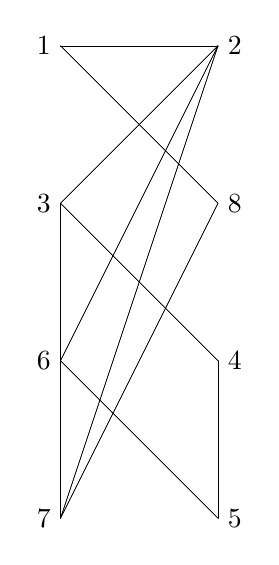
\begin{tikzpicture}[scale=2]
        \tkzDefPoint(0,0){1}
        \tkzDefPoint(1,0){2}
        \tkzDefPoint(0,-1){3}
        \tkzDefPoint(0,-2){6}
        \tkzDefPoint(0,-3){7}
        \tkzDefPoint(1,-1){8}
        \tkzDefPoint(1,-2){4}
        \tkzDefPoint(1,-3){5}
        \tkzDrawSegment(1,2)
        \tkzDrawSegment(1,8)
        \tkzDrawSegment(2,1)
        \tkzDrawSegment(2,3)
        \tkzDrawSegment(2,6)
        \tkzDrawSegment(2,7)
        \tkzDrawSegment(3,2)
        \tkzDrawSegment(3,4)
        \tkzDrawSegment(3,6)
        \tkzDrawSegment(4,3)
        \tkzDrawSegment(4,5)
        \tkzDrawSegment(5,4)
        \tkzDrawSegment(5,6)
        \tkzDrawSegment(6,3)
        \tkzDrawSegment(6,2)
        \tkzDrawSegment(6,5)
        \tkzDrawSegment(6,7)
        \tkzDrawSegment(7,6)
        \tkzDrawSegment(7,2)
        \tkzDrawSegment(7,8)
        \tkzDrawSegment(8,1)
        \tkzDrawSegment(8,7)
        \tkzLabelPoints[left](1,6)
        \tkzLabelPoints[left](3,7)
        \tkzLabelPoints[right](2,8,5)
        \tkzLabelPoints[right](4)
        % \tkzLabelPoints[left,color=orange](1,6)
        % \tkzLabelPoints[left,color=red](3,7)
        % \tkzLabelPoints[right,color=green](2,8,5)
        % \tkzLabelPoints[right,color=orange](4)
      \end{tikzpicture}
            \caption{adjacency graph}\label{fig:adj}
          \end{figure}
    \item The CMK order is \(1,8,7,2,3,4,5,6 \). 
      The matrix graph after permuting according to CMK ordering is as below:

     \[
A =
\begin{pmatrix}
 x & x &   &  x &   &   &   &  \\
x &  x & x &   &   &  &  &   \\
  & x &  x   &  &   &  &   & x  \\
 x &   & x &  x & x &   &   &  x \\
  &   &  x & x &  x & x &   &   x\\
  &  &  & x & x &  x & x &   \\
  &  &   &   &   & x &  x &x \\
 &  &x   &   x&  x &   & x & x 
\end{pmatrix}
\]
\item The reverse CMK order is \(6,5,4,3,2,7,8,1 \). The matrix graph 
  after permuting according to reverse CMK ordering are as following: 
       \[
A =
\begin{pmatrix}
 x & x &   &  x &  x & x  &   &  \\
x &  x & x &   &   &  &  &   \\
  & x &  x   &  &   &  &   &   \\
 x &   & x &  x & x &   &   &   \\
 x &   &  x & x &  x & x &   &   x\\
 x &  &  & x & x &  x & x &   \\
  &  &   &   &   & x &  x &x \\
 &  &   &   &  x &   & x & x 
\end{pmatrix}
\]
\item A multicoloring graph is figure \ref{fig:col}: 
  \begin{figure}[!htbp]
    \centering
      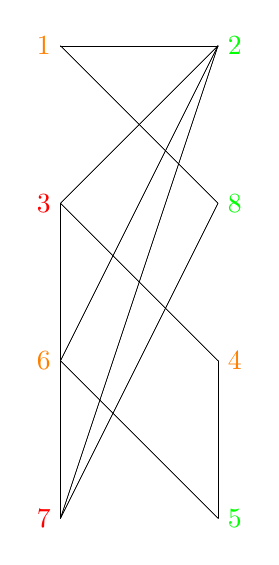
\begin{tikzpicture}[scale=2]
        \tkzDefPoint(0,0){1}
        \tkzDefPoint(1,0){2}
        \tkzDefPoint(0,-1){3}
        \tkzDefPoint(0,-2){6}
        \tkzDefPoint(0,-3){7}
        \tkzDefPoint(1,-1){8}
        \tkzDefPoint(1,-2){4}
        \tkzDefPoint(1,-3){5}
        \tkzDrawSegment(1,2)
        \tkzDrawSegment(1,8)
        \tkzDrawSegment(2,1)
        \tkzDrawSegment(2,3)
        \tkzDrawSegment(2,6)
        \tkzDrawSegment(2,7)
        \tkzDrawSegment(3,2)
        \tkzDrawSegment(3,4)
        \tkzDrawSegment(3,6)
        \tkzDrawSegment(4,3)
        \tkzDrawSegment(4,5)
        \tkzDrawSegment(5,4)
        \tkzDrawSegment(5,6)
        \tkzDrawSegment(6,3)
        \tkzDrawSegment(6,2)
        \tkzDrawSegment(6,5)
        \tkzDrawSegment(6,7)
        \tkzDrawSegment(7,6)
        \tkzDrawSegment(7,2)
        \tkzDrawSegment(7,8)
        \tkzDrawSegment(8,1)
        \tkzDrawSegment(8,7)
        % \tkzLabelPoints[left](1,6)
        % \tkzLabelPoints[left](3,7)
        % \tkzLabelPoints[right](2,8,5)
        % \tkzLabelPoints[right](4)
        \tkzLabelPoints[left,color=orange](1,6)
        \tkzLabelPoints[left,color=red](3,7)
        \tkzLabelPoints[right,color=green](2,8,5)
       \tkzLabelPoints[right,color=orange](4)
      \end{tikzpicture}
      \caption{multicoloring graph}\label{fig:col}
      \end{figure}
The minimum number of colors required is \(3 \).
\item The variant CMK order with starting level \(L_0 \) is \(1,8,7,2,3,6,4,5 \).
  \end{enumerate}
  

\end{solution}
 

\end{document}
